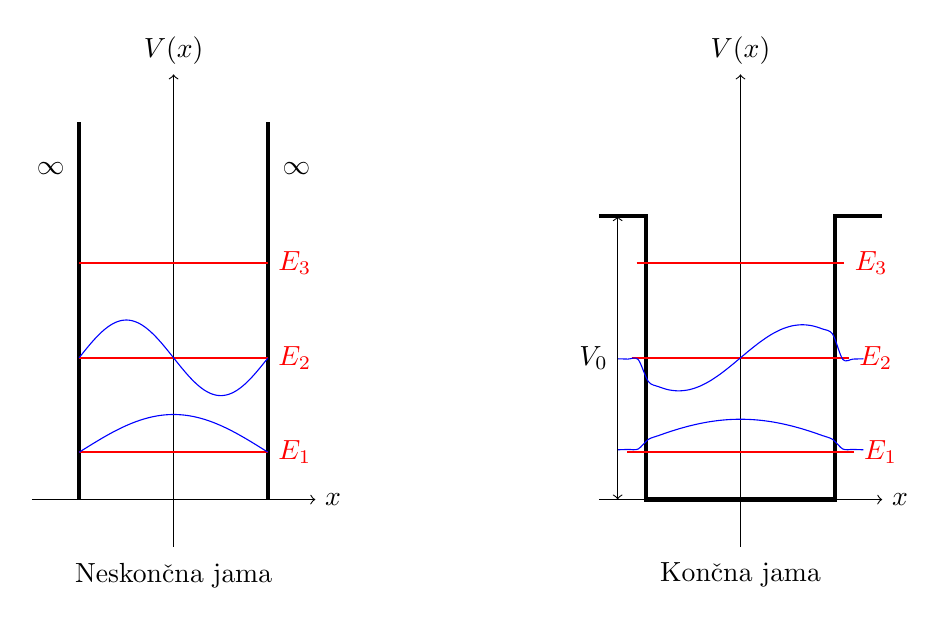
\begin{tikzpicture}[scale=1.2]
    % Infinite Well
    \begin{scope}[xshift=-4cm]
        % Axes
        \draw[->] (-0.5,0) -- (2.5,0) node[right] {$x$};
        \draw[->] (1,-0.5) -- (1,4.5) node[above] {$V(x)$};

        % Walls with infinity symbols
        \draw[ultra thick] (0,0) -- (0,4);
        \draw[ultra thick] (2,0) -- (2,4);
        \node at (-0.3,3.5) {$\infty$};
        \node at (2.3,3.5) {$\infty$};

        % Energy levels with wavefunctions
        \draw[red, thick] (0,0.5) -- (2,0.5) node[right] {$E_1$};
        \draw[blue, smooth, samples=100, domain=0:2]
        plot (\x,{0.5 + 0.4*sin(deg(pi*\x/2))});  % Ground state n=1

        \draw[red, thick] (0,1.5) -- (2,1.5) node[right] {$E_2$};
        \draw[blue, smooth, samples=100, domain=0:2]
        plot (\x,{1.5 + 0.4*sin(deg(pi*\x))});    % First excited n=2

        \draw[red, thick] (0,2.5) -- (2,2.5) node[right] {$E_3$};

        \node at (1,-0.8) {Neskončna jama};
    \end{scope}

    % Finite Well
    \begin{scope}[xshift=2cm]
        % Axes and well structure (unchanged)
        \draw[->] (-0.5,0) -- (2.5,0) node[right] {$x$};
        \draw[->] (1,-0.5) -- (1,4.5) node[above] {$V(x)$};
        \draw[ultra thick] (-0.5,3) -- (0,3) -- (0,0) -- (2,0) -- (2,3) -- (2.5,3);

        % Energy levels with wavefunctions
        \draw[red, thick] (-0.2,0.5) -- (2.2,0.5) node[right] {$E_1$};
        \draw[blue, smooth, domain=-0.3:2.3]
        plot (\x, {0.5 + 0.35*(
                (\x<0)*cos(deg(-1.2))*exp(1.2*(\x-1)) +
                (0<=\x && \x<=2)*cos(deg(1.2*(\x-1))) +
                (\x>2)*cos(deg(-1.2))*exp(-1.2*(\x-1))
                )});

        \draw[red, thick] (-0.15,1.5) -- (2.15,1.5) node[right] {$E_2$};
        \draw[blue, smooth, domain=-0.3:2.3]
        plot (\x, {1.5 + 0.35*(
                (\x<0)*sin(deg(-2.4))*exp(2.4*(\x-1)) +
                (0<=\x && \x<=2)*sin(deg(2.4*(\x-1))) +
                (\x>2)*sin(deg(-2.4))*exp(-2.4*(\x-1))
                )});

        \draw[red, thick] (-0.1,2.5) -- (2.1,2.5) node[right] {$E_3$};

        % V0 arrow from bottom
        \draw[<->] (-0.3,0) -- (-0.3,3) node[midway, left] {$V_0$};

        \node at (1,-0.8) {Končna jama};
    \end{scope}
\end{tikzpicture}